\documentclass{beamer}
\usepackage[utf8]{inputenc}

\usetheme{Madrid}
\usecolortheme{default}
\usepackage{amsmath,amssymb,amsfonts,amsthm}
\usepackage{txfonts}
\usepackage{multicol}
\usepackage{tkz-euclide}
\usepackage{listings}
\usepackage{adjustbox}
\usepackage{array}
\usepackage{tabularx}
\usepackage{gvv}
\usepackage{lmodern}
\usepackage{circuitikz}
\usepackage{tikz}
\usepackage{graphicx}

\setbeamertemplate{page number in head/foot}[totalframenumber]

\usepackage{tcolorbox}
\tcbuselibrary{minted,breakable,xparse,skins}



\definecolor{bg}{gray}{0.95}
\DeclareTCBListing{mintedbox}{O{}m!O{}}{%
  breakable=true,
  listing engine=minted,
  listing only,
  minted language=#2,
  minted style=default,
  minted options={%
    linenos,
    gobble=0,
    breaklines=true,
    breakafter=,,
    fontsize=\small,
    numbersep=8pt,
    #1},
  boxsep=0pt,
  left skip=0pt,
  right skip=0pt,
  left=25pt,
  right=0pt,
  top=3pt,
  bottom=3pt,
  arc=5pt,
  leftrule=0pt,
  rightrule=0pt,
  bottomrule=2pt,
  toprule=2pt,
  colback=bg,
  colframe=orange!70,
  enhanced,
  overlay={%
    \begin{tcbclipinterior}
    \fill[orange!20!white] (frame.south west) rectangle ([xshift=20pt]frame.north west);
    \end{tcbclipinterior}},
  #3,
}
\lstset{
    language=C,
    basicstyle=\ttfamily\small,
    keywordstyle=\color{blue},
    stringstyle=\color{orange},
    commentstyle=\color{green!60!black},
    numbers=left,
    numberstyle=\tiny\color{gray},
    breaklines=true,
    showstringspaces=false,
}
%------------------------------------------------------------
%This block of code defines the information to appear in the
%Title page
\title %optional
{4.2.7}
\date{September 11,2025}
%\subtitle{A short story}

\author % (optional)
{Aditya Appana - EE25BTECH11004}



\begin{document}


\frame{\titlepage}
\begin{frame}{Question}
Find the direction and normal vectors of the line $y-2=0$.
\end{frame}



\begin{frame}[fragile]
    \frametitle{Formulae}

A line can be expressed in two forms:
\begin{align}
\myvec{x\\y} = \myvec{0\\c} + x\myvec{1\\m}
\end{align}
where \myvec{1\\m} is the direction vector of the line and m is the \textbf{slope} of the line.

\begin{align}
{\vec{n}}^{T}x = c
\end{align}
where $\vec{n}$ is the normal vector of the line. \begin{align}{\vec{n}}^T\myvec{1\\m} = 0\end{align}
\end{frame}


\begin{frame}[fragile]
    \frametitle{Solution}

The slope of the line $y-2=0$ is 0, therefore it can be expressed in the first form as:
\begin{align}
\myvec{x\\y} = \myvec{0\\2} + x\myvec{1\\0}
\end{align}\\

Let \myvec{x\\y} be normal vector. Therefore
\begin{align}
\myvec{x\\ y}^T\myvec{1\\0} = 0 \\
x = 0\\
\myvec{x\\y} = \myvec{0\\1}
\end{align}

\end{frame}

\begin{frame}[fragile]
    \frametitle{Solution}
Therefore the line can be expressed as

\begin{align}
\myvec{0\\1}^Tx=2
\end{align}

\vspace{1cm}


Therefore, the direction vector is \myvec{1\\0} , and the normal vector is \myvec{0\\1}.

\end{frame}


\begin{frame}[fragile]
    \frametitle{Python Code}
    \begin{lstlisting}
import matplotlib.pyplot as plt
import numpy as np

fig = plt.figure(figsize = (6,6))
ax = plt.subplot(111)

ax.axhline(y=2, color='r', linestyle='-')

ax.set_ylim(0, 4)
ax.set_xlim(0, 10)

ax.set_xlabel("x-axis")
ax.set_ylabel("y-axis")
ax.set_title("Plot of the Equation y = 2")

ax.grid(True)

plt.show()

\end{lstlisting}

\end{frame}

\begin{frame}
\frametitle{Plot}
\begin{figure}[H]
    \centering
    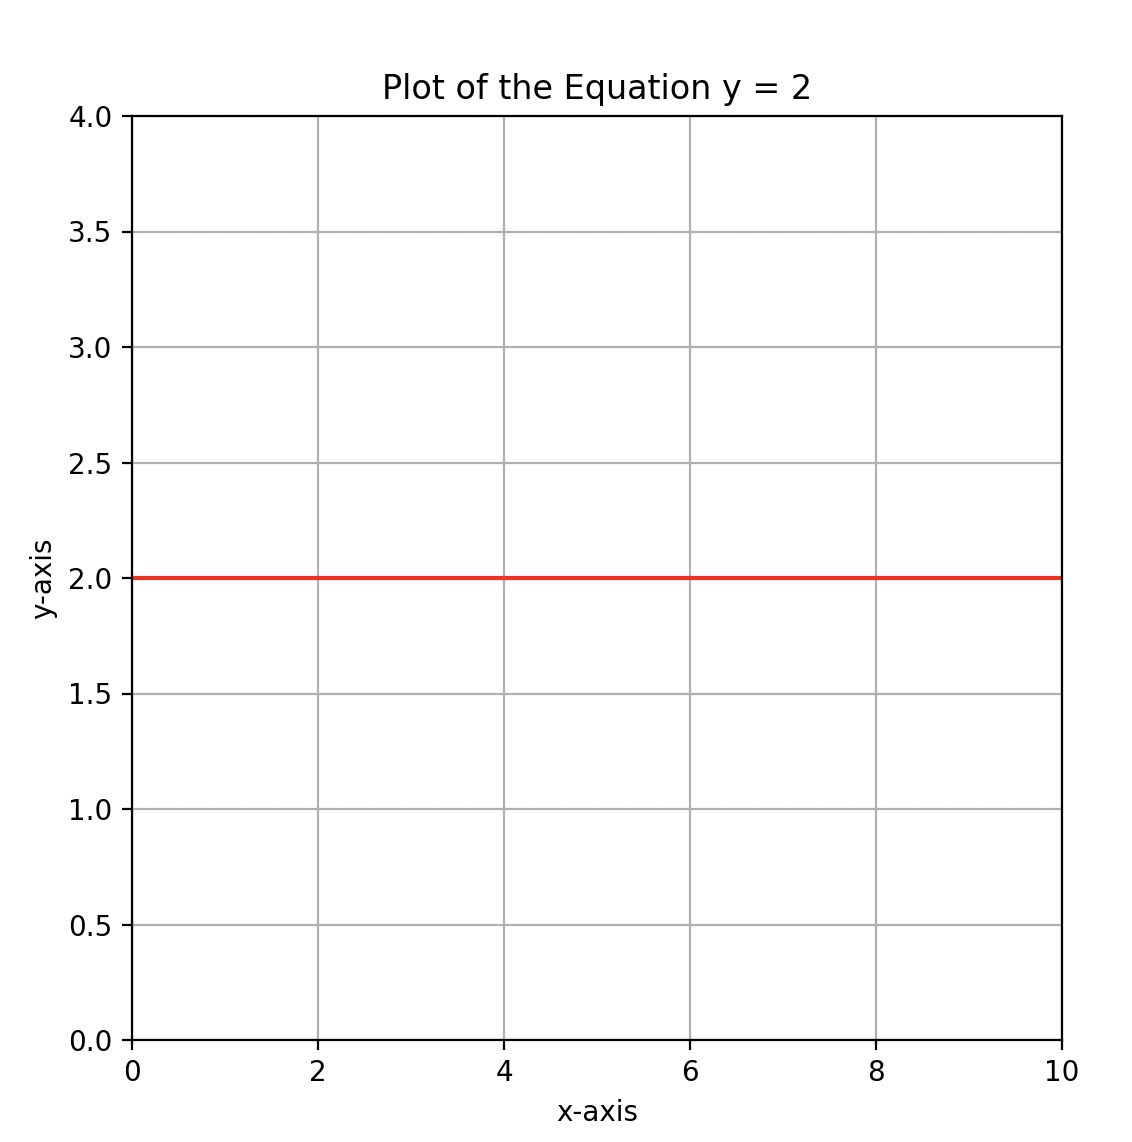
\includegraphics[width=0.6\columnwidth]{Figs/Y=2.png}
    \caption{Plot}
    \label{fig:placeholder}
\end{figure}

\end{frame}



\end{document}